\begin{frame}
	\frametitle{Material}
	
	Material para armar estas slides:
	\begin{itemize}
		\item Cyrill Stachniss - Robot Motion Planning using A*: \url{https://youtu.be/HR1TNa8Lp7w}
		\item Wolfram Burgard - Path and Motion Planning \url{http://ais.informatik.uni-freiburg.de/teaching/ss18/robotics/slides/19-pathplanning-long.pdf}
		\url{http://ais.informatik.uni-freiburg.de/teaching/ss16/robotics/recordings/19-path-and-motion-planning-part1.mp4}
		\url{http://ais.informatik.uni-freiburg.de/teaching/ss16/robotics/recordings/19-path-and-motion-planning-part2.mp4}
		\url{http://ais.informatik.uni-freiburg.de/teaching/ss16/robotics/recordings/19-path-and-motion-planning-part3.mp4}
	\end{itemize}
	
\end{frame}

\begin{frame}
	\frametitle{Motion Planning}
	\note{Información extraída de http://ais.informatik.uni-freiburg.de/teaching/ss18/robotics/slides/19-pathplanning-long.pdf}
	
	Latombe (1991): ``... eminently necessary since, by definition, a robot accomplishes tasks by moving in the real world.''
	
	Objetivos:
	\begin{itemize}
		\item Trayectorias sin colisiones.
		\item El robot debe llegar a la ubicación de destino lo más rápido posible.
	\end{itemize}
\end{frame}

\begin{frame}
	\frametitle{Desafíos}
	\note{Información extraída de http://ais.informatik.uni-freiburg.de/teaching/ss18/robotics/slides/19-pathplanning-long.pdf}
	
	\begin{itemize}
		\item Calcular el camino optimo considerando potenciales incertidumbres en las acciones
		\item Generar rápidamente acciones en el caso de objetos imprevistos
	\end{itemize}
	
\end{frame}


\begin{frame}
	\frametitle{Arquitectura clásica}
	\note{Información extraída de http://ais.informatik.uni-freiburg.de/teaching/ss18/robotics/slides/19-pathplanning-long.pdf}
	
	\begin{figure}[!h]
		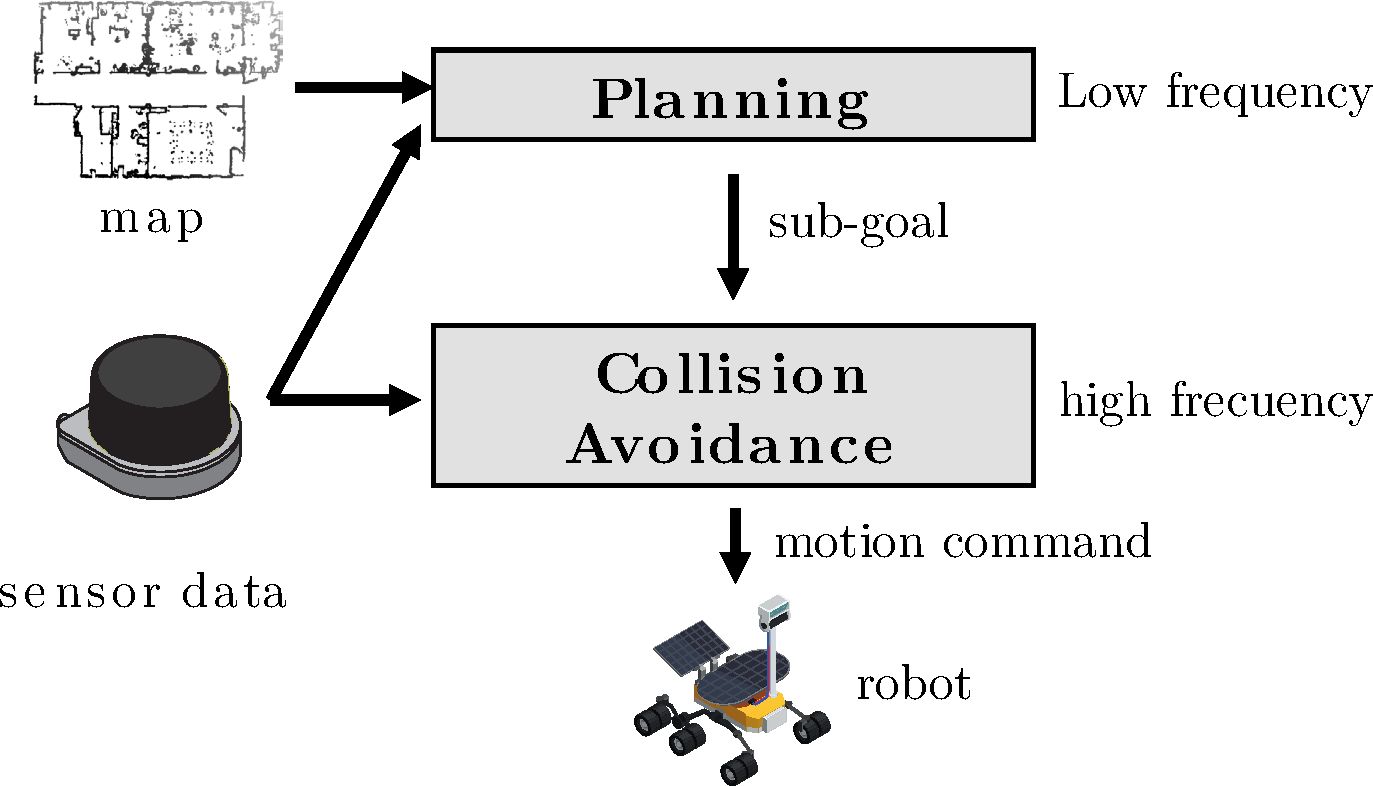
\includegraphics[width=0.8\textwidth]{images/path_planning_architecture.pdf}
	\end{figure}
	
\end{frame}

\begin{frame}
    \frametitle{Arquitectura clásica}
    \note{Información extraída de slides Martin Saska}
    
    \begin{figure}[!h]
        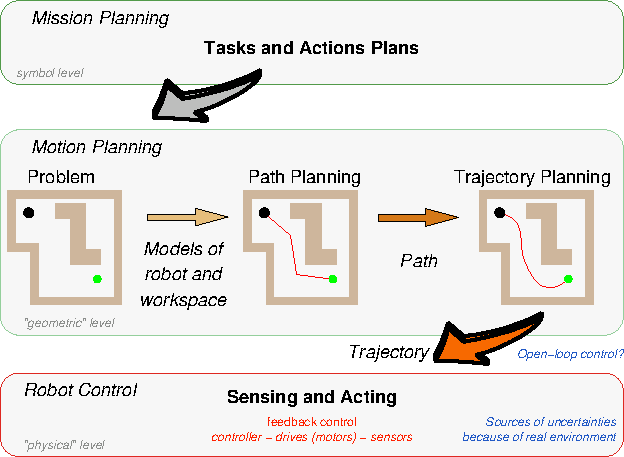
\includegraphics[width=0.5\textwidth]{images/motion_planning_architecture.pdf}
    \end{figure}

    {\bf Motion planning} es parte del ciclo de {\bf mission planning}. Los algoritmos offline se convierten en planificaciones online.
    
\end{frame}


\begin{frame}
	\frametitle{Dynamic Window Approach}
	\note{Información extraída de http://ais.informatik.uni-freiburg.de/teaching/ss18/robotics/slides/19-pathplanning-long.pdf}
	
	
	\TODO{Completar con slides: \url{http://ais.informatik.uni-freiburg.de/teaching/ss18/robotics/slides/19-pathplanning-long.pdf}}
	
	
\end{frame}

\begin{frame}
	\frametitle{Formulación de Motion Planning}
	\note{Información extraída de http://ais.informatik.uni-freiburg.de/teaching/ss18/robotics/slides/19-pathplanning-long.pdf}

	\begin{itemize}
		\item El {\bf problema de la planificación del movimiento} se puede declarar de la siguiente manera. Dado:
		\begin{itemize}
			\item Una pose inicial del robot
			\item Una pose final deseada
			\item Una descripción geométrica del robot
			\item Una representación geométrica del entorno
		\end{itemize}
		\item Encontrar un camino que conduzca al robot gradualmente desde el punto de inicio al punto final sin tocar los obstáculos
	\end{itemize}
\end{frame}

\begin{frame}
	\frametitle{Espacio de configuraciones}
	
	\begin{itemize}
		\item Aunque el problema de planificación de movimiento es 		definido en el mundo regular, vive en otro espacio: el {\bf espacio de configuración}
		\item Una configuración de robot q es una especificación de las posiciones de todos los puntos del robot en relación con un sistema de coordenadas fijo
		\item Por lo general, una configuración se expresa como un vector de posiciones y orientaciones
	\end{itemize}

	
\end{frame}

\begin{frame}
	\frametitle{Espacio de configuraciones}
	\begin{itemize}
		\item Hay dos tipos de regiones: libres u ocupadas (con obstáculos)
		\item Sea $\workSpace = \mathbb{R}^{m}$ el \emph{work space} (para un mundo 2D, $\workSpace = \mathbb{R}^{2}$), $\obstaclesSet \in \workSpace$ el conjunto de obstáculos, $\robotInConfiguration(\robotConfiguration)$ en la configuración $\robotConfiguration \in \configurationSpace$.
        La configuración del robot especifica completamente la pose del robot en $\workSpace$ incluyendo la especificación de todos los grados de libertad. (E.g., un robot con un cuerpo rígido en el plano $\configurationSpace = \begin{bmatrix}
            x & y & \theta
        \end{bmatrix} = \mathbb{R}^{2} \times S_{1}$ .)
        
		\begin{align*}
			 \freeConfigurationSpace &= \left\lbrace \robotConfiguration \in \configurationSpace | \robotInConfiguration(\robotConfiguration) \cap \obstaclesSet =  \emptyset \right\rbrace\\
			 \goalConfiguration &= \configurationSpace / \freeConfigurationSpace
		\end{align*}
	
		\item Definimos:\\
		$\startConfiguration$: configuración \emph{start}\\
		$\goalConfiguration$: configuración \emph{goal}
	\end{itemize}
	
\end{frame}

\begin{frame}
	\frametitle{Ejemplo de espacio de configuraciones}
	
	\begin{figure}[!h]
		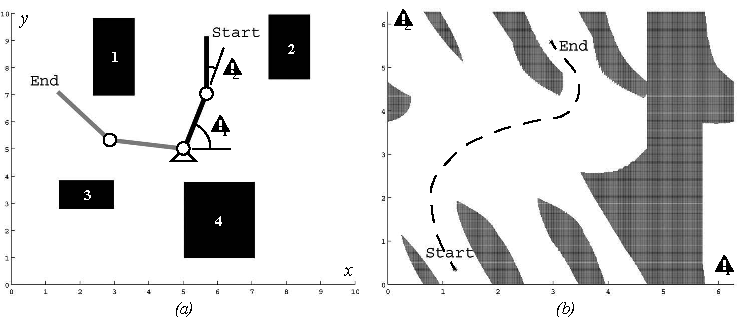
\includegraphics[width=0.8\textwidth]{images/configuration_space_manipulator.pdf}
	\end{figure}
	
\end{frame}

\begin{frame}
    \frametitle{Path vs Trajectory}
    \begin{itemize}
    \item {\bf Path}: es un mapeo continuo en C-space tal que
        \begin{equation*}
            \continuousPath : [0,1] \rightarrow \freeConfigurationSpace \quad \text{con} \quad \continuousPath(0) = \startConfiguration \quad \text{y} \quad  \continuousPath(1) = \goalConfiguration \quad \text{(\emph{solo hay consideraciones goemétricas})}
        \end{equation*} 
    \item {\bf Trajectory} es un camino con una parametrización explícita del movimiento del robot
    \begin{itemize}
        \item Ejemplo: acompañada por una descripción del las leyes de movimiento del robot
            \begin{equation*}
                \motionLaw : [0, 1] \rightarrow \robotActionSpace,
            \end{equation*}
            donde $\robotActionSpace$ es el espacio de acciones del robot. (\emph{incluye la dinámica del robot})
        \end{itemize}
        \vspace{3em}
        \begin{center}
            \alert{El problema de planeamiento consiste en determinar la función $\continuousPath(.)$}  
        \end{center}
    \end{itemize}
\end{frame}

\begin{frame}
    \frametitle{Problema de Motion Planning}
    \note{Información extraída de slides Martin Saska}
    \footnotesize
    Teniendo 
    \begin{itemize}
        \item La dinámica de un sistema con estado $\state$ y $\controlCommand$
        \begin{equation*}
            \dfrac{\partial \state}{\partial t} = f(\state,\controlCommand)
        \end{equation*}
        \item Un conjunto de obstáculos $\obstaclesSet \subset \workSpace$ y un conjunto objetivo $\goalSet \subset \workSpace$     
    \end{itemize}
    El problema de Motion Planning consiste en encontrar el comando de control $\controlCommand$ tal que 
    \begin{equation*}
        \state(t) \notin \obstaclesSet \, \text{para} \,  t \in \mathcal{R}_{+} \, \text{y} \, \state(t) \in \goalSet \,  \forall t \ge T_{f} \, \text{para algún finito} \, T_{f} \geq 0,
    \end{equation*}    
    o, retorna que no existe tal señal de control.
    
    \begin{equation*}
        t \in [T_{0} , T_{f}] \rightarrow i \in [0, 1] : \robotConfiguration(t) = \continuousPath(i) \in \freeConfigurationSpace
    \end{equation*}

    Se pueden agregar requerimientos adicionales como
    \begin{itemize}
        \item Suavizado del camino
        \item Restricciones Kinodynamicas\footnote{La planificación kinodinámica se refiere a la tarea de conducir un robot desde un estado inicial hasta un estado objetivo mientras se evaden los obstáculos y se obedecen las restricciones cinemáticas y dinámicas (en resumen, kinodinámicas) que dictan la relación entre los controles del robot y su movimiento.} (\emph{e.g. considerando fuerzas de fricción})
        \item Criterio de Optimalidad (\emph{e.g. shortest vs fastest})
    \end{itemize}
\end{frame}

\begin{frame}
	\frametitle{Espacio de configuraciones}

	%Espacio de configuraciones es el estado total del robot y el entorno, incluidas las articulaciones y/o movimiento de ruedas)
	
	\begin{figure}[!h]
		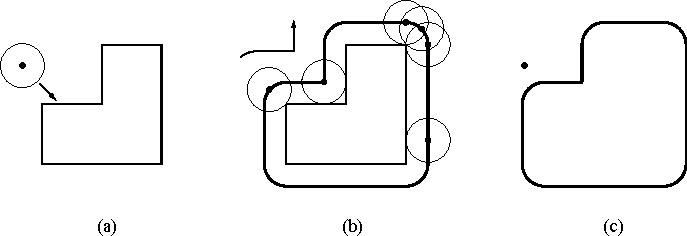
\includegraphics[width=0.8\textwidth]{images/configuration_space_obstacle.pdf}
	\end{figure}
	
\end{frame}

\begin{frame}
	\frametitle{Espacio de configuraciones}
	
	\begin{figure}[!h]
		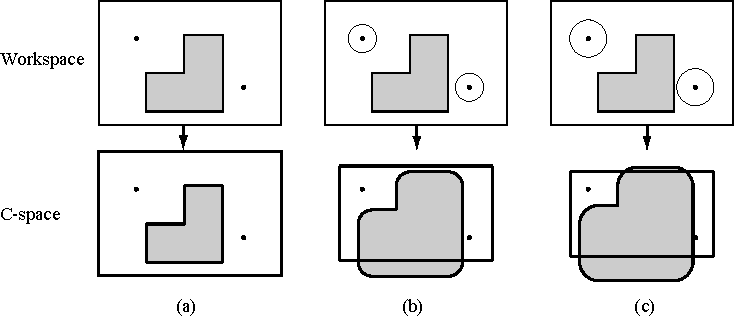
\includegraphics[width=0.8\textwidth]{images/workspace_configuration_space.pdf}
	\end{figure}
	
\end{frame}


\begin{frame}
    \frametitle{Ejemplo de planeamiento sencillo en el C-Space}
    \note{Información extraída de slides Martin Saska}
    
    \begin{figure}[!h]
        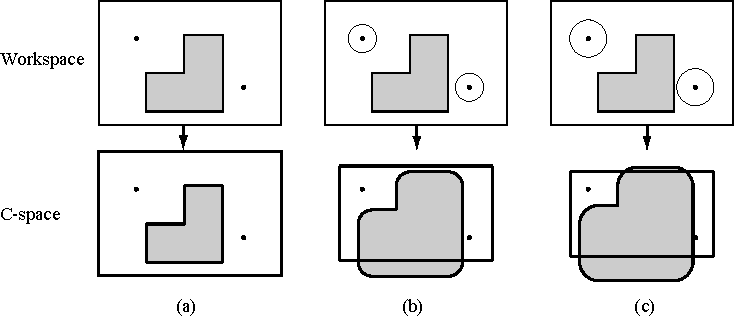
\includegraphics[width=0.8\textwidth]{images/workspace_configuration_space.pdf}
    \end{figure}
    
\end{frame}


\begin{frame}
	\frametitle{Global Planner vs Local Planner}
	
	\begin{figure}[!h]
		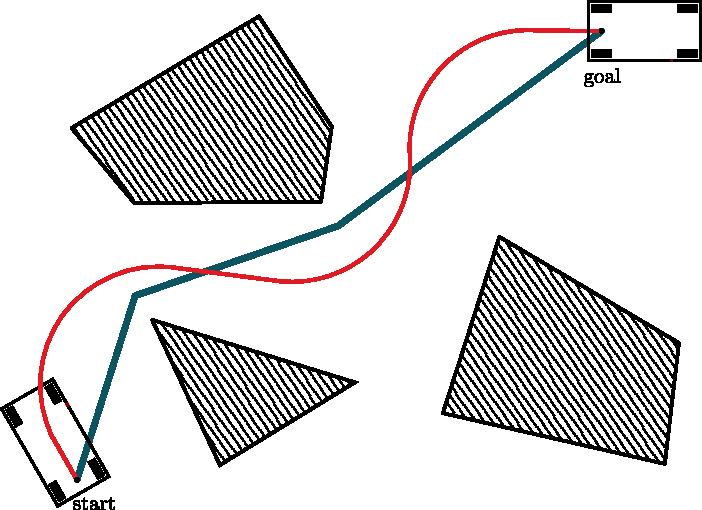
\includegraphics[width=0.5\textwidth]{images/global_local_plan.pdf}
	\end{figure}
	
\end{frame}

\begin{frame}
	\frametitle{Motion Planning Formulation}
	
\end{frame}


%\begin{frame}
%	\frametitle{Planeamiento de movimiento}
%	
%	\begin{block}{Motion Planning}
%		Problema de encontrar rutas sin colisiones a través del espacio de configuraciones. Los obstáculos son convertidos (implícitamente con un verificador de colisiones booleano) al espacio de configuraciones. Se utilizan varios algoritmos geométricos o aleatorios/probabilísticos para buscar a través del espacio de configuraciones un camino desde el principio hasta la meta que no choque con ningún obstáculo.
%	\end{block}
%
%	\begin{block}{Trajectory Planning}
%		Una vez que se tiene un plan de movimiento, este es simplemente un camino geométrico a través del espacio, {\bf no está asociado a un tiempo}. Hay infinitas trayectorias por  cada camino, ya que se puede mover a través del camino con patrones de velocidad variables ilimitados. Durante el planeamiento de movimiento, solo se desea que el movimiento cumpla con algunas restricciones físicas, como qué tan rápido se puede mover el robot y que sea lo más suave posible (por razones de control). Sin embargo, si hay obstáculos dinámicos en el entorno, se tiene que introducir el tiempo en la planificación (el tiempo es una dimensión monótona, es decir, solo puede avanzar, no retroceder). Entonces, el camino debe especificar el momento correcto; de lo contrario, el camino no será válido porque el robot podría colisionar con algunos de los objetos dinámicos.
%	\end{block}
%
%	\begin{block}{Path Planning}
%	Un camino NO es igual a una trayectoria. Una trayectoria es un camino con información adicional de cómo se atravesar dicho camino con respecto al tiempo, es decir tiene información de velocidad.
%	\end{block}
%\end{frame}


\begin{frame}
	\frametitle{Rapidly Exploring Random Trees (RTTs)}
	
\end{frame}

\begin{frame}
	\frametitle{Road Map Planning}
	
\end{frame}


\begin{frame}
	\frametitle{Generalized Voronoi Diagram}
	
\end{frame}

\begin{frame}
	\frametitle{Voronoi Diagram}
	
\end{frame}

\begin{frame}
	\frametitle{Randomized Road Maps}
	
\end{frame}

\begin{frame}
	\frametitle{From Road Maps to Paths}
	
\end{frame}

\begin{frame}
	\frametitle{Randomized Road Maps}
	
\end{frame}

\begin{frame}
	\frametitle{Randomized Road Maps}
	
\end{frame}

\begin{frame}
	\frametitle{Randomized Road Maps}
	
\end{frame}

\begin{frame}
	\frametitle{Randomized Road Maps}
	
\end{frame}

\begin{frame}
	\frametitle{Markov Decision Process}
	
\end{frame}

